\section{Further Studies on Original LIBERO}
\label{supp:legacy}
This section reports two studies of $\pi_{0.5}$ on original LIBERO, each with its own tasks, start states and unit of analysis. Both back Sec.~\ref*{M-sec:sensitivity} of the main paper (the size of a change is not its cost): the ten-condition study (Sec.~\ref{supp:legacy-d3}) and the headlight-versus-matched-dimming comparison (Sec.~\ref{supp:legacy-d2}).

\subsection{Command change ranks conditions by success change, but not task--condition cells}
\label{supp:legacy-d3}
Does a larger command change mean a larger loss of success? Across conditions, yes: a condition's mean command change ranks its mean success change with rank correlation $-0.903$ $[-0.952,-0.309]$ over the ten condition means. Across the 400 task--condition cells, the correlation is $-0.075$ $[-0.195,+0.043]$, an interval that includes zero (Table~\ref{tab:legacy-aggregation-readout}). This supports Sec.~\ref*{M-sec:sensitivity} of the main paper: the command change orders conditions but hardly tells which tasks lose success.

\paragraph{Data: 2,344 of 2,400 planned pairs.}
The study runs ten persistent visual conditions on 40 tasks, two start states and three policy-noise draws. Paired internal measurements and outcomes are available for 2,344/2,400 planned perturbed/clean pairs: 2,110 joint successes, 104 lost successes, 83 gained successes and 47 joint failures. Of the 400 task--condition cells, 364 have six pairs, 20 have four and 16 have five; missing pairs remain missing. The 236 observed clean episodes are reused across conditions with their original outcome labels.

\paragraph{What is measured, and when.}
Unlike the main paper's first-query measure, features and commands are taken at two scheduled mid-episode controls: 20/40 for Spatial, 25/55 for Object, 30/60 for Goal and 50/100 for LIBERO-10, at the first generation step and relative to a clean evaluation of the same state. The command change uses the first five planned commands (translation part, 15 numbers). The L18 response magnitude is the relative RMS over five positions and 1,024 channels. Main-camera conditional total variation (TV) of attention requires all eight heads. The two steps are averaged within each episode, and each outcome is counted once. Condition means weight episodes equally within condition; cell means are ranked equally. The lost-success AUROCs compare lost successes (SF) with joint successes (SS) within conditions and weight the 21,405 SF--SS comparisons, not tasks.

\begin{table}[t]
\centering\small
\caption{\textbf{The command change ranks condition means by success change, but not task--condition cells.} Ten-condition study, 2,344 perturbed/clean pairs, 40 tasks, ten conditions; each scalar is averaged over two observations. First two rows: rank correlation between the mean command change (translation part) and the mean success change, across the ten condition means and across the 400 task--condition cells. Last three: lost-success AUROC, comparing lost with kept successes within conditions and weighting SF--SS pairs, unlike the task-equal AUROC of Sec.~\ref{sec:supp-bounded-internal}. Estimates use case-level scalars; the correlation intervals in the text come from the same 1,000 whole-task draws (40 tasks resampled with replacement, each carrying its start states, noises, conditions and shared clean episodes; ranks recomputed; percentile intervals with linear interpolation).}
\label{tab:legacy-aggregation-readout}
\setlength{\tabcolsep}{3pt}
\begin{tabular}{p{0.76\columnwidth}r}
\toprule
Comparison & Estimate\\
\midrule
Command change--success change, condition means & $-0.903$\\
Command change--success change, task--condition cells & $-0.075$\\
L18-response lost-success AUROC & $0.535$\\
Main-camera conditional-TV lost-success AUROC & $0.581$\\
Command-change lost-success AUROC & $0.421$\\
\bottomrule
\end{tabular}
\end{table}

\paragraph{Within conditions, response size barely separates lost from kept successes.}
All three lost-success AUROCs are near chance ($0.5$); the command-change AUROC is below it, so within a condition, pairs that lose a success have, if anything, smaller command changes than pairs that keep it.

\paragraph{After removing task and condition effects, the internal measures co-vary but hardly predict success.}
We rank each variable globally with average ties and remove additive task and condition effects. Pearson correlation of the residual ranks is $0.722$ between L18 response and command change, $0.401$ between L18 response and main-camera TV, and $0.286$ between main-camera TV and command change. Their correlations with the success change $\Delta Y$ are $-0.0009\ [-0.0422,0.0395]$, $-0.0280\ [-0.0694,0.0194]$ and $+0.0542\ [0.0093,0.0998]$ for L18 response, main-camera TV and command change. Intervals use 1,000 draws of 40 task clusters that keep nested states, noises, conditions, missing pairs and reused clean episodes, without suite stratification or multiplicity adjustment. These coefficients describe association in the observed data after removing additive task and condition effects.

\paragraph{Attention mass and attention shape carry different associations.}
A separate first-query comparison on the same 2,344 pairs centers percentile ranks within condition. The signed change of main-camera attention mass correlates $-0.00351$ with the command change; a Jensen--Shannon (JS) summary of the attention distribution correlates $+0.493$. Both average the first five positions over ten generation steps, three layers and eight heads; unlike conditional TV, JS pools layers. Both are point estimates without intervals.

\paragraph{Implementation notes.}
Commands are in adapter coordinates; acknowledgements of execution are recorded separately. Both bootstrap analyses use seed 20261008.

\subsection{Headlight removal and a dimming matched in image statistics}
\label{supp:legacy-d2}
Removing the headlight changes the first five commands 5.12 times as much as a global dimming matched in initial image statistics, yet both succeed on 77/80 cases, each on two cases where the other fails. This supports Sec.~\ref*{M-sec:sensitivity} of the main paper: a fivefold larger command change comes with the same success count, and equal counts hide changed outcomes.

\paragraph{Fivefold command change, equal success counts, exchanged failures.}
The command change is the RMS of the 15 translation coordinates of the first five commands. Its mean is 0.0570 for headlight removal and 0.0111 for matched dimming (ratio of means 5.12); the paired difference is $0.0459\ [0.0363,0.0562]$ (95\% interval over task clusters), and the headlight change is larger on 76 cases and smaller on four. The paired success difference is $0\ [-5,5]$ pp; this interval describes the observed comparison, and an equivalence test was not prespecified.

\paragraph{Data and runs.}
The study has 80 cases from 40 tasks and start states 10/11, each run clean, with the headlight off and with matched dimming. Each run succeeds on 77 of 80 cases, and each pair of runs shares one failure (75 joint successes, 2 and 2 single failures, 1 joint failure). The runs share the start state and ten settling steps, checked before the first query.

\paragraph{The dimming is matched on initial image statistics only.}
Initial RGB images have shape $256\times256\times3$. For each camera, matching uses the image mean and the mean absolute difference from clean. A gain $g\in\{0.25,0.275,\ldots,0.75\}$ is chosen to minimize the largest of the four statistic mismatches, ties going to the larger gain. Dimming scales the ambient, diffuse and specular RGB of the active lights, including the headlight, and uses no policy output or outcome. All 80 cases meet the criterion of five code values and stay in the analysis: the largest mismatch is 3.94, gains lie in [0.35,0.55], and each gain stays fixed for the episode. Spatial lighting patterns and later images can still differ.

\begin{figure*}[t]\centering
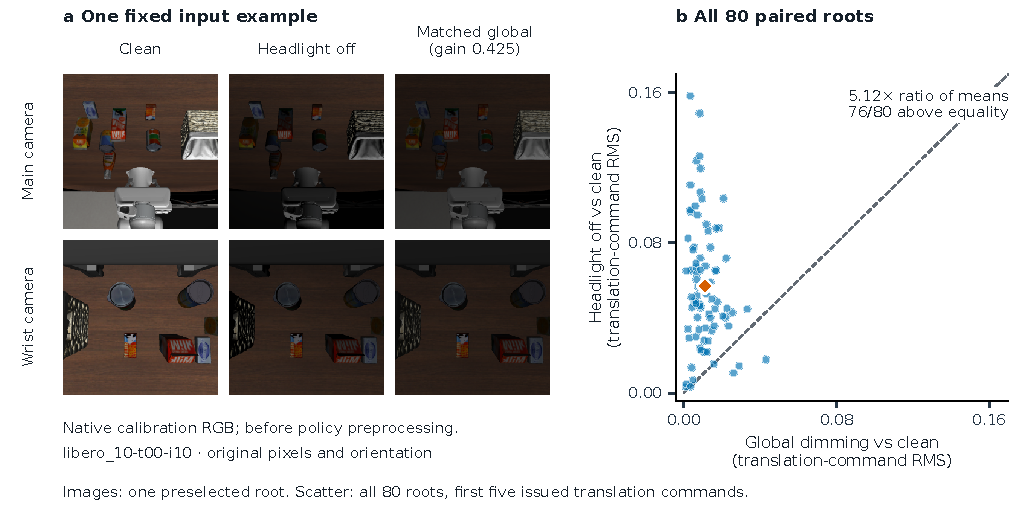
\includegraphics[width=\textwidth]{figures/supp_legacy_d2_inputs_print_v2.pdf}
\caption{\textbf{Images matched in summary statistics can still change the commands differently.} Main and wrist images of the first complete case in fixed order (LIBERO-10 task 0, start state 10, global gain 0.425), chosen by order, not by response or outcome; pixels and orientation as recorded. The command comparison in the text uses all 80 cases and the RMS over 15 translation coordinates, in command units rather than displacement.}
\label{fig:legacy-d2-inputs}
\end{figure*}
